%Introduction
\label{intro}
Modelling sanitary sewer network flows allow cities to understand and solve issues that impact its society, environment and economy. To model sanitary sewer network flows, it is first necessary to identify the behavior of the system. As described by \citet{Vallabhaneni2007} the flows in the network usually have two different behaviors that are classified as: 1. dry-weather flow (DWF); 2. wet-weather flow (WWF). To apply a continuous simulation and successfully forecast the flows in the sanitary sewer system, the model should be able to account for both DWF and WWF.

Typically, DWF pattern can be estimated by analyzing historical data from flow measurements available along the network or at the downstream end during dry periods \cite{Bennett1999}. Intuitively, usually more water is discharged into the sewer in day time than during the night. More complexity is added when trying to estimate WWF in the sanitary sewer network. Flow increases in the network due to inflow and infiltration often trigged by rainfall or snowmelt. This incremental quantity of flow which finds its way into the sanitary sewer network during a rainfall event is known by Rainfall Dependent Inflow and Infiltration (RDII).

The challenge on RDII estimations lies upon the different ways stormwater enters a sanitary or combined sewer \cite{Mosley2001}. Stormwater can inflow to the sanitary or combined sewer network directly through foundation and roof drains connections, leaky manhole covers, or stormwater drains.  Infiltration occurs due to defects in the network components such as: damaged pipes, joints, manholes, etc. \cite{Rossman2016}
Quantity of inflow and infiltration (I\&I) increases proportionally with intensity of the rainfall and snowmelt. Urban areas located in cold climate can have a significant inflow due to snowmelt and was, therefore, considered during this study. For that, the incremental flow caused by snowmelt will be referred here as Snowmelt Dependent Inflow and Infiltration (SDII). Event-based Inflow and Infiltration (EBII) will be used as a general term for both snowmelt and rainfall inflow and infiltration.


\begin{figure}[ht]
    \centering
	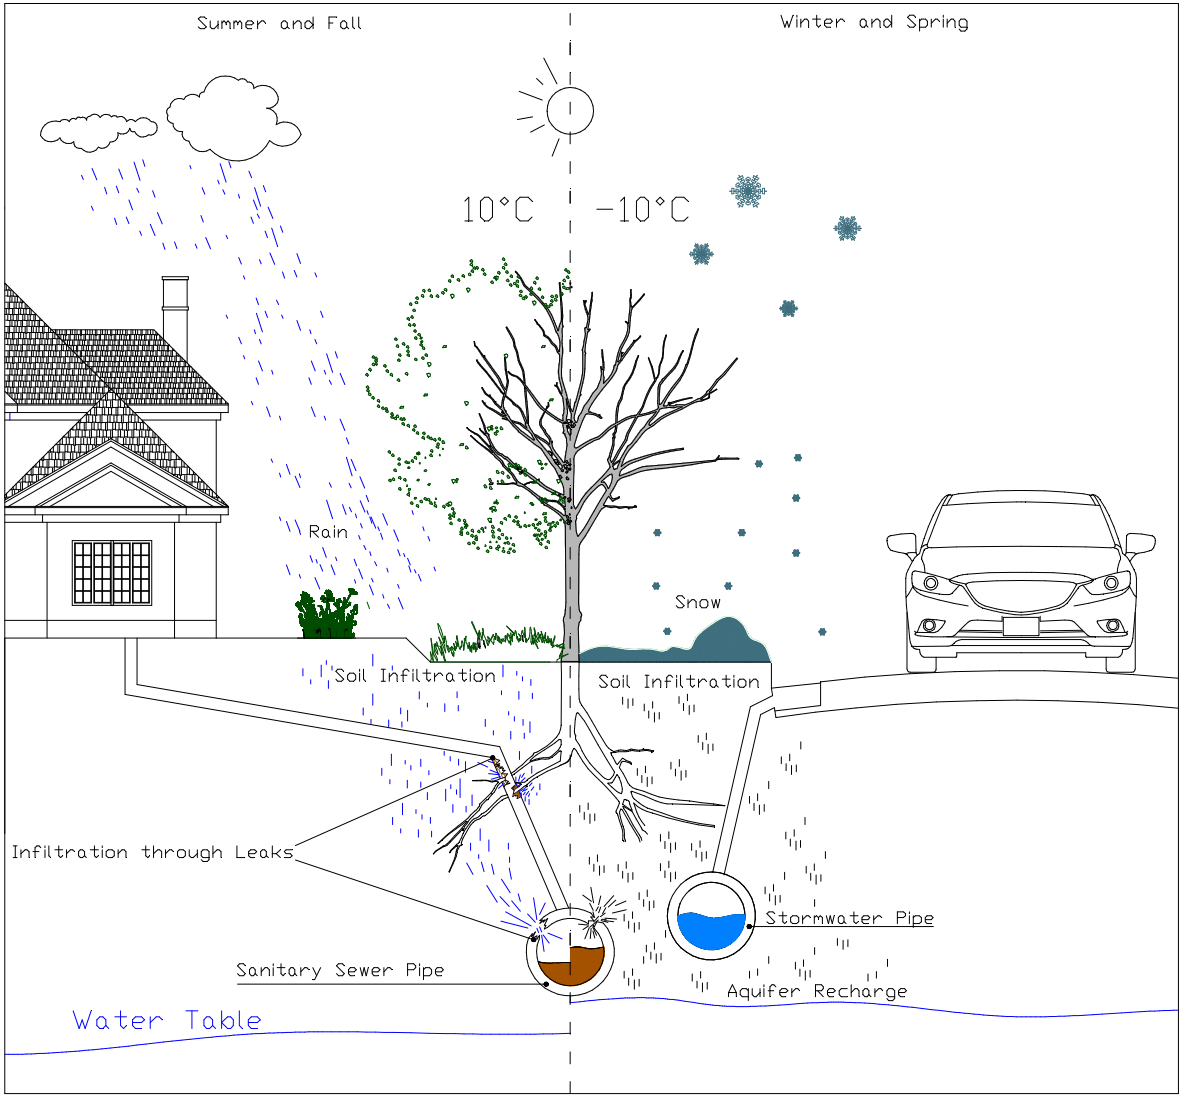
\includegraphics[scale=0.62]{figures/sanitary_sewer_leakage.png}
	\caption{Wet-weather Infiltration}
	\label{fig:wetinf}
\end{figure}


\section{Motivation}
Event-base inflow and infiltration (EBII) causes increase of the quantity of flow into sanitary sewer systems. This increase may cause sanitary sewer overflow (SSO) due to exceedance of the system capacity  \cite{Rossman2016}. In some cities, sanitary sewer is combined with stormwater sewer network. The capacity of this coupled systems may also be exceeded during an event causing combined sewer overflow (CSO) \cite{Vallabhaneni2007}. When the capacity is exceeded, untreated water rejected by the wastewater treatment plants (WWTPs) is released into surface waters \cite{DeRodaHusman2016} such rivers and streams. Upstream capacity-related issues may cause wastewater to find its way into basements or streets \cite{Roesner2009}. Untreated water released on the surface water bodies or urban area increases the risk of human contamination by infectious diseases. 
Although these are well known problems, they are still present in urban centers around the globe. Frequency of CSOs are seasonal dependent. The current prediction of more frequent intensive rainfall events also increases the frequency of CSO \cite{DeRodaHusman2016} and enlarge the damage caused by these overflows. Moreover, wastewater overflows can cause conflicts in the society when streams or rivers are used both as an option to dispose wastewater and recreational area as described by \citet{heikkinen2016}. To give cities, municipalities and water utilities the ability to predict SSOs and CSOs is one of the motivations of this study. However, other benefits are also aimed. A continuous simulation considering urban hydrology and hydraulics can also be used to improve the service and reduce operational costs for water utilities. 
EBII can increase the inflow of wastewater to WWTPs for weeks due to possible long response times \cite{Mosley2001}. Obviously, the operational cost of the plant will increase since more wastewater needs to be treated. A continuous simulation might be able to identify increases over time on the flow pattern in specific pipes or sub-divisions of the network. This would be an indicator for the water utility to carry further inspections and evaluate whether the infrastructure is damaged allowing infiltration. Furthermore, a digital model of the network gives to the water utilities the ability to analyze the impacts on the whole network caused by changes in the network such as: decommissioning of a water tower, changing pumping schedule, or analyzing impacts of a future new neighborhood. 


%TELL ABOUT SIMILAR PROJECTS \cite{Body2013}, \cite{}, in compenhagen and etc


